% \chapter{Introduction}
\chapter{Multiscale Analysis of the Wetting Phenomena on Doped 2D
  Materials}
\label{ch:wet}
\renewcommand*\imgdir{img/wet/}

% \dictum[Samuel T. Coleridge \textit{The Rime of the Ancient Mariner}]{%
% Water, water, every where.
  % }%
% \worktodo{find the quote or quit}

\vspace{1em}

\chapterabstract{This chapter is adapted from the following journal
  article: Tian, T., Lin, S., Li, S., Zhao, L., Santos, E. J. G., \&
  Shih, C.-J. Doping-Driven Wettability of Two-Dimensional Materials:
  A Multiscale Theory. Langmuir 33, 12827–12837 (2017). }


\section{Introduction}
\label{sec:wet-intro}

Engineering molecular interactions at two-dimensional (2D) materials
interfaces enables new technological opportunities in functional
surfaces and molecular epitaxy.
%
Understanding the molecular epitaxy and wettability of 2D
materials represents the crucial first step towards quantifying the
interplay between the interfacial forces and electric potential of 2D
materials interfaces.
%
An accurate determination of the interfacial tension of even
commonly-studied materials like graphene and 2H-MoS\textsubscript{2},
remains highly disputed
\autocite{taherian2013what,Kozbial_2015_wetting_mos2,Parobek_2015_wetting_rev,Govind_Rajan_2016}.
%
As briefly introduced in \autoref{sec:van-der-waals}, early studies on
the surface science of 2D materials has highlighted the effects of the
airborne contaminants
\autocite{li_2013_airborne,Xu_2013_withwhat,Kozbial_study_2014_gr_wetting,Kozbial_2015_wetting_mos2,Chow_2015_wetting_WS2}
and the underlying substrate
\autocite{Raj_2013_wetting_rev,rafiee_2012_transparency,Shih_2012_prl,shih_2013_wetting_natmat},
since the length scale for the van der Waals (vdW) radius is
comparable to the thickness of a monolayer. On the other hand, a
subtle but important fact is that the 2D semimetals (e.g, graphene and
silicene) and 2D semiconductors (e.g., transition metal
dichalcogenides (TMDCs)) possess low density of states (DOS) around
the intrinsic Fermi level (\(E_{\mathrm{F}}\)), such that the effect
of doping, either induced by the surroundings
\autocite{Chen_2013_doping,Varchon_2007_elec_struc_gr_SiC,Giovannetti_2008_doping},
or by the electrostatic gating
\autocite{Das_2008_doping,Perera_2013_doping}, also comes into
play. Recent advance in the \textit{ab initio} calculations and
scanning tunneling microscopy (STM) studies on the adsorbed molecules
on graphene
\autocite{Muruganathan_2015_tunable_vdw_gr,Huttmann_2015_vdw_gr_doping}
has provided some clues to the doping-dependent vdW
interactions. Subsequently, the doping-induced change in the
wettability of graphene has been observed in several contact-angle (CA)
experiments
\autocite{Hong_2016_mechanism,goniszewski_correlation_2016,Ashraf_2016_doping},
and molecular dynamics (MD) simulations
\autocite{Ostrowski_2014_tunable,Ren_2015_interfacial,Taherian_2015_asym_EW,Daub_2007_nanoscale_EW}.
%
In this respect, however, most reports described the doping-dependent
wettability with the basic Young-Lippmann equation (YLE)
\autocite{Lippmann_1875_wetting}. The interplay between the orientation of
liquid molecules at the interface \autocite{Shen_2006_lifshitz_water} and
the electronic structure of the 2D materials is often ignored. In
order to address the discrepancies among the literature, a general and
complete theoretical picture that bridges the gap between different
length scales, is clearly required.


In this chapter, we propose a multiscale theoretical framework to model
the change of interfacial tension between liquid and a sheet of
monolayer 2D material.
%
Multiscale physical phenomena are considered,
as shown in \autoref{fig:wet-scheme-method}. At the atomistic scale
(several \AA{}), we formulate the dependence of surface energy of a 2D
material on the doping density using the quantum capacitance (QC)
calculated by density functional theory (DFT). Next, the
surface-charge-induced reorientation of liquid molecules adjacent to
the interface is associated with an $N$-body system, which is resolved
by molecular dynamics (MD) simulations, allowing quantification of the
interfacial tension in the absence of electrolytes in liquid at the
molecular scale (\(10^{0} \sim 10^{1}\) nm).
%
The effect of the electrical
double layer (EDL) induced by the electrostatic interactions between
the 2D material surface charges and the ionic species in liquid, is
further addressed at the continuum level (\(10^{0} \sim 10^{4}\) nm).
%
Practical
considerations, such as the defect density and the surface
contamination are also taken into account to provide a comprehensive
understanding of the phenomena. Finally, we examine and validate our
theory by comparing with the contact angle changes reported in the
electrowetting and the substrate-induced doping experiments.

\begin{figure}[htbp]
  \centering
  \import{\imgdir}{TOC.pdf_tex}
% \includegraphics[width=0.95\linewidth]{../img/scheme-methods.pdf}
  \caption{\label{fig:wet-scheme-method} Scheme of the proposed
    multiscale approach for modeling the doping-induced wettability
    tuning of 2D materials. }
\end{figure}

\section{Results and Discussions}
\label{sec:wet-results}

\subsection{Surface Energy of Doped 2D Materials}
\label{sec:wet-gamma-doped}

The studies in this chapter focus on the thermodynamic wetting
properties.
%
Consider a liquid (\emph{L}) droplet sitting on a flat,
monolayer 2D material (\emph{2D}) which is supported by a solid substrate,
following the Young’s equation, the change of the equilibrium contact
angle \(\theta\) upon doping, is given by
\begin{equation}
\label{eqn:wet-def-Young-Delta-theta}
\gamma_{\mathrm{L}} \Delta \cos\theta = \Delta \gamma_{\mathrm{2D}}
                                 - \Delta \gamma_{\mathrm{2D-L}}
\end{equation}
where \(\gamma_{\mathrm{L}}\) and \(\gamma_{\mathrm{2D}}\) are the
surface tensions of liquid and the 2D material considered,
respectively, \(\gamma_{\mathrm{2D-L}}\) is the interfacial tension
between the liquid and the contacting 2D material. We define
\(\Delta \gamma = \gamma - \gamma_{0}\) for all the surface
(interfacial) tensions considered and
\(\Delta \cos \theta = \cos \theta - \cos \theta_{0}\), where the
index 0 corresponds to the case of an intrinsic 2D material with the
doping density per unit area \(\sigma_{\mathrm{2D}} = 0\).
%
In the
theoretical analysis presented here, we aim to model
\(\Delta \cos \theta\) as a function of \(\sigma_{\mathrm{2D}}\). Note
that under the assumptions that (i) the change of \(E_{\mathrm{F}}\)
in the doped 2D materials does not result in the interfacial electron
transfer with liquid (\ie no electro\-chemical reactions), (ii) the doping
does not alter the surface energy of the underlying substrate,
and (iii) the vdW and electrostatic interactions are perfectly
additive and pairwise, the effect of the underlying
substrate can be decoupled.
%
Due to these assumption, the debate “wetting transparency”
\autocite{rafiee_2012_transparency,shih_2013_wetting_natmat} as discussed in \autoref{sec:diel-prop-2d}, does not
affect our analysis of \(\Delta \cos \theta\), which is independent of
\(\gamma_{0}\) or \(\theta_{0}\).
%
Moreover, as pointed out in \autoref{ch:vdw}, the conventionally
assumed wetting transparency may be questionable due to many-body vdW
effects. As a results, in this chapter, we do not focus on the
absolute value of wettability and contact angle, but rather its change
upon doping in the 2D material layer.

First, we model the dependence of \(\gamma_{\mathrm{2D}}\) on the doping
level. Consider a closed, constant-pressure and constant-volume system
containing a sheet of free-standing 2D material, following the Euler
homogeneous function theorem of thermodynamics, the total internal
energy of the system \(U\), is given by \(U = TS + \mu_{\mathrm{2D}} N +
\gamma_{\mathrm{2D}} A + \psi_{\mathrm{2D}} q\)
\autocite{Bard_1980_electrochem_book}, where \(T\) is the temperature, \(S\) is
the entropy, \(\mu_{\mathrm{2D}}\) is the chemical potential of the 2D
material per unit lattice, \(N\) is the number of unit lattices, \(A\) is
the area of the 2D material, and \(\psi_{\mathrm{2D}}\) and \(q\) are the
electric potential and total charge in the 2D material,
respectively. At constant \(T\), combining with the first law of
thermodynamics and the differential form of \(U\), it follows:
\begin{equation}
\label{eqn:wet-dgamma-dpsi}
\mathrm{d} \gamma_{\mathrm{2D}} = -\frac{q}{A} \mathrm{d} \psi_{\mathrm{2D}}
                                = -\sigma_{\mathrm{2D}} \mathrm{d} \psi_{\mathrm{2D}}
\end{equation}
relating the surface tension change of a free-standing 2D material as
a function of its doping density \(\sigma_{\mathrm{2D}}\).
%
After bringing a tiny amount of charge
\(q\) from infinity to the charge-neutral 2D material in the
aforementioned system, and combining the quantum capacitance $C_{\mathrm{Q}}$ (see \autoref{sec:qc-field-effect-transp}),
the surface energy change is therefore given
by:
\begin{equation}
\label{eqn:wet-delta-gamma-sigma-free-2D}
\Delta \gamma_{\mathrm{2D}} = - \int_{0}^{\psi_{\mathrm{2D}}} \sigma_{\mathrm{2D}} \mathrm{d}\psi'
                            = - \int_{0}^{\sigma_{\mathrm{2D}}} \sigma' \left( \frac{1}{C_{\mathrm{Q}}}\right) \mathrm{d} \sigma'
\end{equation}
where
% \(C_{\mathrm{Q}} = \mathrm{DOS}(E_{\mathrm{F}}) e^{2}\) is the quantum
% capacitance of the 2D material
% \autocite{Davies_1997_book,Das_Sarma_2011_electron_gr},
\(\psi_{\mathrm{2D}} = -(E_{\mathrm{F}} - E_{\mathrm{F,0}})/e\) and
\(E_{\mathrm{F,0}}\) corresponds to the Fermi level of the 2D material
at the charge neutral point (CNP). Accordingly, eq
\autoref{eqn:wet-delta-gamma-sigma-free-2D} provides a simple relation which
depicts the surface tension change of a 2D material at the
quantum-mechanical level.
%
The DOS as a function of \(E_{\mathrm{F}}\) for a variety of 2D
materials using the density functional theory are calculated using the
procedures in \autoref{ch:qc}, with the following 2D materials
considered: TMDC monolayers (2H-MX\(_{\text{2}}\), M = Mo, W and X =
S, Se, Te, the phase 2H is omitted for the rest of this chapter),
silicene, germanene, phosphorene (monolayer black phosphorus), and
graphene.  The doping density in a 2D material is calculated according
to their quantum capacitances (see \autoref{ch:qc}).

\begin{figure}[!htbp]
  \centering
  \import{\imgdir}{dgamma-sigma.pgf}
% \includegraphics[width=0.75\linewidth]{../img/dgamma-sigma.pdf}
\caption{\label{fig:wet-dgamma-sigma} Atomistic scale effect on surface tension:
  \(\Delta \gamma_{\mathrm{2D}}\) as a function of
  \(\sigma_{\mathrm{2D}}\) for selected 2D materials: graphene,
  silicene, germanene, phosphorene, MoS\(_{2}\), MoSe\(_{2}\),
  MoTe\(_{2}\), WS\(_{2}\), WSe\(_{2}\) and WTe\(_{2}\). The 2D
  semimetals (graphene, silicene and germanene) with low high quantum
  capcitances show larger decrease of \(\gamma_{\mathrm{2D}}\) upon
  doping, compared with the 2D semiconductors (TMDCs, phosphorene).}
\end{figure}

\autoref{fig:wet-dgamma-sigma} presents the calculated
\(\Delta \gamma_{\mathrm{2D}}\) as a function of
\(\sigma_{\mathrm{2D}}\) for the 2D materials considered
here.
%
Clearly, the doping of 2D materials reduces their surface
energy, or based on the classical definition, the work required to
separate two stacked monolayers is lowered.
%
Among the 2D materials at
the same doping level, we find that graphene shows the highest degree
of surface energy decrease, up to -16 mJ\(\cdot \mathrm{m}^{-2}\) , or
\textasciitilde{}20\% reduction of its intrinsic surface tension
\autocite{shih_2013_wetting_natmat}, when \(\sigma_{\mathrm{2D}}\) =
\(\pm 4\times10^{13}\ e\cdot \mathrm{cm}^{-2}\).
%
A clear trend is that the surface energy decrease is more significant
in the 2D semimetals (e.g. graphene, silicene, and germanene) compared
with the 2D semiconductors (e.g. TMDCs) due to the different
electronic structures (parabolic vs Dirac dispersion, see
\autoref{sec:qc-gener-behav-2deg}).
%
This reflects the fact that the effective mass of carriers in the 2D
semiconductors is much higher than that in the 2D semimetals
\autocite{Davies_1997_book}, thereby resulting in high DOS, as well as a
high \(C_{\mathrm{Q}}\) (see eq
\autoref{eqn:wet-delta-gamma-sigma-free-2D}). This concept also
explains why the surface energy decrease for silicene and germanene
are lower than that for graphene \autocite{Yan_2013_e-hv-couple}.  To our
knowledge, the doping-induced surface energy change in 2D materials
has never been investigated experimentally, which may be of interest
for future study, inspired by the advances in direct measurement of 2D
material surface energy \autocite{van_Engers_2017_direct_surf_gr}. Note
that for modeling the macroscopic wetting behavior on a doped 2D
material interface, the reorientation of liquid molecules and the EDL
effect also need to be taken into account.
%
As will be discussed
in following sections, the doped-induced change of \(\gamma_{\mathrm{2D}}\) does not
imply a reduced wettability, because the quantum capacitance effect
also reduces the interfacial tension, \(\gamma_{\mathrm{2D-L}}\),
which yields zero net effect on wettability.

The interactions between 2D materials and liquid will be discussed in
the following sections. In a doped 2D material, the delocalized carriers
are confined in the 2D plane. Therefore, following the spirit of the
mean-field theory, we treat it as a continuously, uniformly charged
surface. Since these charges are either generated by interacting with
the underlying substrate, or electrostatically induced by gating, the
electroneutrality still holds before in contact with liquid.
%
The surface charges result in two consequences that may change
\(\gamma_{\mathrm{2D-L}}\), including (i) the reorientation of
adjacent liquid molecules \autocite{Ostrowski_2014_tunable} and (ii) the
formation of the electric double layer (EDL) at the liquid-solid
interface, known as the electrowetting effect
\autocite{Lippmann_1908,Mugele_2005_EW_rev}. Under the assumption that the
vdW and electrostatic (Coulombic) interactions which compose the
interfacial tension are additive, we propose that the interfacial
tension change is given by:

\begin{equation}
\label{eqn:wet-delta-gamma-decompose}
\Delta \gamma_{\mathrm{2D-L}} = \Delta \gamma_{\mathrm{2D-L}}^{\mathrm{Orien}}
                              + \Delta \gamma_{\mathrm{2D-L}}^{\mathrm{EDL}}
\end{equation}
where \(\Delta \gamma_{\mathrm{2D-L}}^{\mathrm{Orien}}\) and \(\Delta
\gamma_{\mathrm{2D-L}}^{\mathrm{EDL}}\) refer to the contributions
from the reorientation and the EDL effects, respectively.
%
We also
assume that \(\Delta \gamma_{\mathrm{2D-L}}^{\mathrm{Orien}}\) is independent of
the electrolyte concentration, since the concentration of liquid
molecules is typically orders-of-magnitude higher.



\subsection{Reorientation of Liquid Molecules}
\label{sec:wet-reorien}

First we consider the orientation effect. Understanding the
reorientation effect involves positioning and sampling the collective,
time-averaged motion of liquid molecules near the interface, a
standard molecular dynamics (MD)
problem~\autocite{Israelachvili_2011_book}.
%
Note even with the
state-of-the-art MD algorithms, it still remains challenging to accommodate
the calculations for the EDL, in which the length scale of electric
field can be larger than one micrometer in diluted electrolyte
solutions.
% e.g., pure water with self-ionized
% H\(_{\text{3}}\)O\(^{\text{+}}\) and OH\(^{\text{-}}\) ions.
Here we consider the graphene-water interface as a model system. The
MD simulations were performed with the help from Prof. Shangchao Lin
in Florida State University, US and Prof. Lingling Zhao in
Southeastern University, China.
%
In order to precisely determine the interfacial interactions using MD
simulations, instead of the commonly used models that compared the
nanoscale contact angle by placing a nano\-droplet onto a sheet of
suspended 2D material
\autocite{Ostrowski_2014_tunable,Daub_2007_nanoscale_EW,Ren_2015_interfacial,Taherian_2015_asym_EW},
we simulate the difference of the total potential energy,
\(E\), between two separate systems:
\begin{enumerate}
\item System L: only water molecules with two surfaces exposing to vacuum
  
\item System GL: the same amount of water molecules as in L, with one
  surface in contact with graphene (placed at z = 0) and the other
  surface exposing to vacuu
\end{enumerate}
%
The two simulation systems can be seen in \autoref{fig:wet-MD-res1}\lc{a}.
%
As stated above, that the current model can only reveal the static and
macroscopic wetting behavior, while the effects of dynamic properties
or surface roughness, as discussed by some recent MD-based
nano-electrowetting studies \autocite{Yuan_2010_PF,Zhao_2015_pillar}, are
not considered.
%
The total energy in both systems
can be formulated as:
\(E_{\mathrm{L}} = \mu_{\mathrm{L}}n_{\mathrm{L}} +
2\gamma_{\mathrm{L}}S\) and
\(E_{\mathrm{GL}}=\mu_{\mathrm{L}}n_{\mathrm{L}}+(\gamma_{\mathrm{L}}
+ \gamma_{\mathrm{2D-L}} + \gamma_{\mathrm{2D}})S\), respectively,
where \(\mu_{\mathrm{L}}\) is the chemical potential per water
molecule in the bulk phase, \(n_{\mathrm{L}}\) is the number of liquid
molecules in the simulation box, and \(S\) is the area of the 
\emph{xy}-plane of the unit cell.
%
One can show that
\(E_{\mathrm{GL}} - E_{\mathrm{L}} = (\gamma_{\mathrm{2D-L}} +
\gamma_{\mathrm{2D}} - \gamma_{L})S = (\Phi + 2
\gamma_{\mathrm{2D}})S\), where \(\Phi\) is the interfacial adhesion energy,
which is defined as
\(\Phi = \gamma_{\mathrm{2D-L}} - \gamma_{\mathrm{2D}} -
\gamma_{\mathrm{L}}\).
Combining with eq
\autoref{eqn:wet-def-Young-Delta-theta}, the change of interfacial
energy \(\Delta \Phi\) is written as:
\begin{equation}
\label{eqn:wet-Delta-Phi-Delta-cos}
\Delta \Phi = \Delta (E_{\mathrm{GL}} - E_{\mathrm{L}})/S - 2\Delta \gamma_{\mathrm{2D}} = -\gamma_{\mathrm{L}} (\Delta \cos \theta)^{\mathrm{Orien}}
\end{equation}
where \((\Delta\cos \theta)^{\mathrm{Orien}}\) corresponds to the
contact angle change due to the reorientation effect.
%
Note that in the
current MD simulation framework, the surface tension of the 2D material
remains unchanged (i.e.  \(\Delta \gamma_{\mathrm{2D}}=0\)), since the
Fermi level change with respect to \(\sigma_{\mathrm{2D}}\) (see eq
\autoref{eqn:wet-delta-gamma-sigma-free-2D}) is not included in the algorithm.
%
When analyzing the reorientation effect on the MD level, we adopt the
water surface tension value of
\(\gamma_{\mathrm{L}}=63.6\ \mathrm{mJ}\cdot \mathrm{m}^{-2}\) in the
SPC/E model \autocite{Vega_2007_tension}.
%
Note that the value of
\(\gamma_{\mathrm{L}}\) only affects the results of
\(\Delta \cos \theta\) while not the interaction potential \(\Phi\), as revealed by eq
\autoref{eqn:wet-Delta-Phi-Delta-cos}.
%
Moreover, even though the surface tension $\gamma_{\mathrm{L}}$ from
SPC/E model is $\sim{}$12.6\% lower than the experimental value (72.8
mJ\(\cdot\)m\(^2\)), such minor difference does not affect our
conclusion.
%
Accordingly, \(\Delta \Phi\) follows
\(\Delta \Phi = \Delta (E_{\mathrm{GL}} - E_{\mathrm{L}})/S = \Delta
\Phi_{\mathrm{LJ}} + \Delta \Phi_{\mathrm{Coul}}\), where
\(\Delta \Phi_{\mathrm{LJ}}\) and \(\Delta \Phi_{\mathrm{Coul}}\)
correspond to the change for the vdW and Coulombic interaction
potentials, respectively.

\begin{figure}[!htbp]
  \centering
  \import{\imgdir}{MD_phi_plot.pgf}
% \includegraphics[width=0.9\linewidth]{../img/fig-pot-dens.pdf}
  \caption{\label{fig:wet-MD-res1}%
    Molecular scale influence on interfacial
    energy. \textbf{a}. Geometry of the periodic MD simulation box for
    water molecules only (L) and water-graphene (GL) systems, with
    \textasciitilde{} 27000 water molecules per unit cell.
    %
    \textbf{b}. Change
    of total adhesion energy \(\Delta\Phi\), and its partial
    contributionsfrom Lennard-Jones \(\Delta\Phi_{\mathrm{LJ}}\) and
    Coulombic \(\Delta\Phi_{\mathrm{Coul}}\) interactions, as a
    function of \(\sigma_{\mathrm{2D}}\). The filled regions indicate
    the error margin of calculation. \(10^{-3}\) \textit{e}/atom
    corresponds to a charge density of
    \(3.80 \times 10^{12}\ e \cdot \mathrm{cm}^{-2}\).}
\end{figure}


\autoref{fig:wet-MD-res1}\lc{b} shows the
calculated \(\Delta \Phi\) and its contributions from the
Lennard-Jones (\(\Delta \Phi_{\mathrm{LJ}}\)) and Coulombic
interactions (\(\Delta \Phi_{\mathrm{Coul}}\)), as functions of
\(\sigma_{\mathrm{2D}}\).
%
We observe that the change of adhesion energy
in the doped graphene system is dominated by the Coulombic
interaction.
%
When the doping level of graphene is
\(\pm 4 \times 10^{13}\ e\cdot \mathrm{cm}^{-2}\), the Coulombic
interaction causes a decrease in the adhesion energy of
\textasciitilde{} -15 mJ\(\cdot \mathrm{m}^{-2}\).
%
On the other hand, the vdW
interaction only causes a slight increase in the
adhesion energy by less than 5 mJ\(\cdot \mathrm{m}^{-2}\).
%
In other
words, concerning the reorientation of water molecules at large doping
levels, the Coulombic interaction favors the decrease of
\(\gamma_{\mathrm{2D-L}}\) as well as the contact angle \(\theta\),
while the vdW interaction slightly increases both
\(\gamma_{\mathrm{2D-L}}\) and \(\theta\).
%
We shall note that due to
the highly polar nature of water molecules, the average
inter-molecular equilibrium distance in the absence of external
electric field (\(r_{\mathrm{O-O}}=2.75\ \mathrm{\AA}\)) is shorter
than the Lennard-Jones equilibrium distance
(\(r_{\mathrm{O-O}}=3.16\ \mathrm{\AA}\))
\autocite{Mark_2001_MD_water}.
%
Increasing the doping density of the
graphene sheet essentially enhances the Coulombic attractions between
graphene and water molecules, further reducing the inter-molecular
equilibrium distance, which eventually leads to a slight increase in
\(\Delta \Phi_{\mathrm{LJ}}\).
%
% This can be revealed by the distance between the first
% water layer and graphene (calculated from maximal
% \(\rho_{\mathrm{L}}\) from \autoref{fig:wet-MD-res}(d), which slightly
% decreases in doped graphene systems, compared with the charge-neutral
% system,
The plot of \(\Delta \Phi\) as a
function of \(\sigma_{\mathrm{2D}}\) in \autoref{fig:wet-MD-res1}\lc{a}
shows an asymmetric behavior.
%
This can be further revealed from the \emph{z}-dependent local
molecular density \(\rho_{\mathrm{L}}\) and charge density
\(\delta_{\mathrm{L}}\) profiles of the water molecules, as shown in
\autoref{fig:wet-MD-res2}\lc{a} and
\autoref{fig:wet-MD-res2}\lc{b}, respectively.
%
\begin{figure}[!htbp]
\centering
\import{\imgdir}{MD_density.pgf}
\caption{\label{fig:wet-MD-res2} Density and charge profiles in the MD
  simulations. \textbf{a} and \textbf{b} are the local density
  \(\rho_{\mathrm{L}}\) and local charge density
  \(\delta_{\mathrm{L}}\) of water molecules as a function of distance
  \(z\) from graphene surface in the MD simulation corresponding to
  \autoref{fig:wet-MD-res1}, respectively.}
\end{figure}

The molecular density of the first water layer adjacent
to graphene increases when graphene is p-doped
(\(\sigma_{\mathrm{2D}}=0.012\ e\cdot \mathrm{cm}^{-2}\), or
equivalently 4.56 \textit{e}/atom) and decreases when graphene is
n-doped (\(\sigma_{\mathrm{2D}}=-0.012\ e\cdot \mathrm{cm}^{-2}\), or
equivalently -4.56 \textit{e}/atom) compared with the case of
charge-neutral graphene, indicating the polarity-dependent adsorption
of water molecules on graphene: lighter H atoms prefer to adsorb onto
n-doped graphene electrostatically.
% Similar trend can also be observed
% in the \(\delta_{\mathrm{L}}\) (\autoref{fig:wet-MD-res}(e))and water
% dipole orientation \(\cos \mu\) (S1) profiles, both suggesting that
% water orientation depends strongly on \(\sigma_{\mathrm{2D}}\): more
% negative \(\sigma_{\mathrm{2D}}\) tends to orient the water dipoles
% more towards the 2D interface, reflected by the more positive charge
% densities due to first-layer H atoms, and the more negative
% \(\cos \mu\) values.
%
Interestingly, the
\(\Delta \Phi_{\mathrm{Coul}}\) exhibits small positive contribution
for slightly n-doped graphene, when
\(\sigma_{\mathrm{2D}} \approx -2\times10^{13}\ e\cdot
\mathrm{cm}^{-2}\) or equivalently -0.76 \textit{e}/atom, indicating
that the reorientation of interfacial water molecules by small
negative charges on graphene helps minimizing the Coulombic
interactions.
% The trend observed in hydrogen-bond densities (see S3)
% also matches those observed in \(\rho_{\mathrm{L}}\),
% \(\delta_{\mathrm{L}}\) and \(\cos \mu\) profiles.

% Finally, we believe that the asymmetric behavior of \(\Delta
% \Phi_{\mathrm{Coul}}\) with respect to \(\sigma_{\mathrm{2D}}\) is due to
% the nonlinear decrease in \(\delta_{\mathrm{L}}\) of the first water
% layer, when graphene becomes more n-doped (see S2(d)).  As a
% general trend, \(\delta_{\mathrm{L}}\) of the first water layer
% increases when \(\sigma_{\mathrm{2D}}\) becomes more negative, due to
% the attraction of H atoms to the graphene surface. However we observe
% a decrease of \(\delta_{\mathrm{L}}\) when \(\sigma_{\mathrm{2D}}\)
% ranges from -0.001 to -0.006 \(e \cdot \mathrm{cm}^{-2}\) (see 
% S2(d)), which could be a combined result of the graphene-water
% Coulombic interactions and intermolecular hydrogen bonding. We also
% notice a nonlinear behavior in the \(\rho_{\mathrm{L}}\) of the first
% water layer: when \(\sigma_{\mathrm{2D}}\) becomes more negative, the
% interatomic distance \(r_{\mathrm{C-O}}\) between graphene C and water O
% atoms will increase due to Coulombic repulsion.  Note that the
% increased Coulombic repulsion energy for C−O pairs from more negative
% \(\sigma_{\mathrm{2D}}\) values is balanced by the increased vdW
% attractions between C−O pairs when \(r_{\mathrm{C-O}}\) increases, which
% eventually prevents the reduction of the first water layer density at
% an equilibrium C-O distance, as seen at \(\sigma_{\mathrm{2D}} < -0.01\
% e \cdot \mathrm{cm}^{-2}\) (S2(b)). Here we propose a simple
% capacitor-like model, considering the contributions from
% \(\delta_{\mathrm{L}}\) of the first water layer of the first water
% layer and \(\sigma_{\mathrm{2D}}\) to the interfacial Coulombic energy
% \(\Phi_{\mathrm{Coul}}^{\mathrm{int}}\) (see the discussion in
% Supporting Information and S4). We show that in the n-doped graphene system
% the charge density of the first water layer has a major contribution
% to \(\Delta \Phi_{\mathrm{Coul}}\). The nonlinear behavior of
% \(\delta_{\mathrm{L}}\) at low n-doping level is responsible for the
% shift of maximum of the \(\Delta
% \Phi_{\mathrm{Coul}}-\sigma_{\mathrm{2D}}\) curve. The analysis further
% indicates the importance of interfacial water configuration in
% determining the change of the interaction potentials.

Although the MD simulation results show that the Coulombic
interactions between the doped graphene and water molecules dominate
the reorientation effect, such conclusion may not be readily applied
to other types of 2D materials, as the intensity of vdW interactions
and surface charge polarization can vary greatly. First, the
microscopic vdW and Coulombic interactions on 2D materials depend on
the lattice constant and atomic density. In addition, for homoatomic
2D materials such as graphene, silicene, germanene and phosphorene,
their surface charge polarization is negligible compared to
heteroatomic 2D materials, for instance TMDC. It has been shown that,
for TMDCs, the value of \(\gamma_{\mathrm{2D-L}}\) is already largely
determined by the Coulombic interactions in the charge-neutral systems
\autocite{Govind_Rajan_2016,Chow_2015_wetting_WS2}. Therefore we anticipate that
case-by-case studies and DFT calculations which deal with the
post-doping charge redistribution, might be required, as shown by
several previous studies
\autocite{Sresht_2015,Govind_Rajan_2016,Sresht_2017_mos2-liquid}.


\subsection{Electrical Double Layer Effect}
\label{sec:org492fdee}

The EDL effect that decreases the interfacial tension has been
extensively studied in the context of the electrowetting phenomena
\autocite{Mugele_2005_EW_rev}, in which the interfacial tension is reduced due to
the adsorption of ionic species at the solid-liquid interface.
%
Here we
extend such concept to the 2D material-liquid systems.
%
Consider a
closed system containing an interface formed between liquid and a
sheet of free-standing 2D material, by combining with the Gibbs
adsorption theory~\autocite{Bard_1980_electrochem_book}, one obtains:
\begin{equation}
\label{eq:wet-gibbs}
\mathrm{d} \gamma_{\mathrm{2D-L}}^{\mathrm{EDL}} = -\sigma_{\mathrm{2D}} \mathrm{d} \psi_{\mathrm{2D}}
                                                   -\sum_{\mathrm{i}} \Gamma_{\mathrm{i}} \mathrm{d}\mu_{\mathrm{i}}
\end{equation}
where \(\Gamma_{\mathrm{i}}\) and \(\mu_{\mathrm{i}}\) are the interfacial
excess and the chemical potential of the ionic specie \(i\) at the
interface, respectively. Relative to that in the bulk phase
(\(\psi=0\)), the interfacial chemical potential of a charged solute
\(\mu_{\mathrm{i}}\), is given by
\(\mu_{\mathrm{i}}=z_{\mathrm{i}}e\psi_{\mathrm{2D}}\), where
\(z_{\mathrm{i}}\) is the valency of component \(i\), under the assumption
that the interfacial electric potential is equal to
\(\psi_{\mathrm{2D}}\). As with the approach leading to
\autoref{eqn:wet-delta-gamma-sigma-free-2D}, it follows:
\begin{equation}
\label{eqn:wet-Delta-gamma-2DL-EDL-full}
\Delta \gamma_{\mathrm{2D-L}}^{\mathrm{EDL}} = 
-\int_{0}^{\sigma_{\mathrm{2D}}} \sigma' \left(\frac{1}{C_{\mathrm{Q}}}\right) \mathrm{d}\sigma'
-\int_{0}^{\sigma_{\mathrm{L}}} \sigma' \left(\frac{1}{C_{\mathrm{EDL}}}\right) \mathrm{d}\sigma'
\end{equation}
where \(\sigma_{\mathrm{L}}\) is the interfacial charge density per unit
area in the liquid phase, and \(C_{\mathrm{EDL}}\) is the EDL
capacitance.
%
Combining \autoref{eqn:wet-Delta-gamma-2DL-EDL-full} with eqs
\autoref{eqn:wet-def-Young-Delta-theta} and \autoref{eqn:wet-delta-gamma-sigma-free-2D},
the contact angle change due to the EDL effect, \((\Delta \cos
\theta)^{\mathrm{EDL}}\) is given by:
\begin{equation}
\label{eqn:wet-Delta-cos-EDL}
(\Delta \cos \theta)^{\mathrm{EDL}} = -\frac{1}{\gamma_{\mathrm{L}}}
                                      \int_{0}^{\sigma_{\mathrm{L}}} \sigma' 
                                      \left(\frac{1}{C_{\mathrm{EDL}}}\right) \mathrm{d}\sigma'
\end{equation}
In other words, \autoref{eqn:wet-delta-gamma-sigma-free-2D} and
\autoref{eqn:wet-Delta-gamma-2DL-EDL-full} suggest that \(\sigma_{\mathrm{2D}}\)
decreases both \(\gamma_{\mathrm{2D}}\) and \(\gamma_{\mathrm{2D-L}}\) to
the same extent, i.e. \(\int_{0}^{\sigma_{\mathrm{2D}}}
\sigma'/C_{\mathrm{Q}} \mathrm{d}\sigma'\), such that the contribution
of quantum capacitance cancels out in the YLE.
%
This is not surprising as the contact angle described by YLE only
depends on the change of interfacial adhesion, instead of absolute
surface tensions.

For a \(z:z\) electrolyte solution, with the molar concentration
\(c_{0}\) and the electrolyte valence \(z\), we describe the electric
potential $\psi$ profile in liquid with the one-dimensional
Gouy-Chapman-Stern (GCS) model \autocite{Stern_1924_theory}, as schematically
shown in \autoref{fig:wet-EDL-scheme}.
%
\begin{figure}[!htbp]
  \centering
  \import{\imgdir}{scheme-EDL.pdf_tex}
% \includegraphics[width=0.5\linewidth]{../img/2d-ph-dependency+MD.pdf}
  \caption{\label{fig:wet-EDL-scheme} Scheme of the interface between
    the 2D material and the aqueous phase in the continuum model of
    EDL.}
\end{figure}
The EDL consists of a
Helmholtz layer with the permittivity of liquid
\(\varepsilon_{\mathrm{L}}\) and thickness \(d_{\mathrm{H}}\), next to
the Gouy-Chapman (GC) diffuse layer where the electric potential
profile follows the Poisson-Boltzmann equation
\autocite{Bard_1980_electrochem_book}.
%
The \(C_{\mathrm{EDL}}\) of the
GCS model is equivalent to two capacitors in series,
namely,
\begin{equation}
\label{eqn:wet-GCS-capacitance-series}
\frac{1}{C_{\mathrm{EDL}}} = \frac{1}{C_{\mathrm{H}}} + \frac{1}{C_{\mathrm{GC}}}
\end{equation}
where \(C_{\mathrm{H}}=\varepsilon_{\mathrm{L}}/d_{\mathrm{H}}\) is the
capacitance of the Helmholtz double layer and
\(C_{\mathrm{GC}}=\sqrt{\frac{2z^{2}e^{2}\varepsilon_{\mathrm{L}}c_{0}N_{\mathrm{A}}}{k_{\mathrm{B}}T}}
\cosh(\frac{ze\psi_{\mathrm{GC}}}{2k_{\mathrm{B}}T})\) is the
differential capacitance of the GC layer, with \(\psi_{\mathrm{GC}}\)
corresponding to the electric potential at the GC interface.
%
Consider
a Gaussian enclosure including the 2D material layer and the EDL, due
to a zero net electric field at the surface of the Gaussian enclosure,
the electroneutrality of the system \autocite{Bard_1980_electrochem_book}
suggests:
\begin{equation}
\label{eqn:wet-neutrality}
\sigma_{\mathrm{2D}} + \sigma_{\mathrm{L}} = 0
\end{equation}
And therefore, the electric potentials corresponding to the surface of
the 2D material and the outer Helmholtz plane, \(\psi_{\mathrm{2D}}\)
and \(\psi_{\mathrm{GC}}\), are given by:
\begin{equation}
\label{eqn:wet-psi-GC}
\begin{aligned}
  \psi_{\mathrm{GC}} &= -\frac{2k_{\mathrm{B}}T}{ze} 
                         \sinh^{-1}\left(
                         \frac{-\sigma_{\mathrm{2D}}}{\sqrt{8c_{0}N_{\mathrm{A}}\varepsilon_{0}\varepsilon_{\mathrm{L}}k_{\mathrm{B}}T}}
                            \right) \\
  \psi_{\mathrm{2D}} &= \psi_{\mathrm{GC}} + \sigma_{\mathrm{2D}}\frac{d_{\mathrm{H}}}{\varepsilon_{0}\varepsilon_{\mathrm{L}}}
\end{aligned}
\end{equation}
where \(N_{\mathrm{A}}\) is the Avogadro constant and \(k_{\mathrm{B}}\)
is the Boltzmann constant. Accordingly, the final form
of \((\Delta \cos \theta)^{\mathrm{EDL}}\) is given by:
\begin{equation}
\label{eqn:wet-Delta-cos-EDL-final}
\begin{aligned}
(\Delta \cos \theta)^{\mathrm{EDL}} &= \frac{\sigma_{\mathrm{2D}}^{2}}{2\gamma_{\mathrm{L}}
                                       C_{\mathrm{H}}}\frac{1}{\gamma_{\mathrm{L}}}
                                       \sqrt{\frac{32k_{\mathrm{B}}^{3}T^{3} \varepsilon_{0}\varepsilon_{\mathrm{L}} c_{0} 
                                       N_{\mathrm{A}}}{z^{2}e^{2}}} 
                                       \left[\cosh(\frac{z e \psi_{\mathrm{GC}}}{2k_{\mathrm{B}} T}) -1 \right]\\
                                    &= \frac{\Delta \sigma_{\mathrm{2D}}^{2}}{2\gamma_{\mathrm{L}}}
                                       \left[ \frac{1}{C_{\mathrm{H}}} + \frac{1}{(C_{\mathrm{DH}} + 
                                       C_{\mathrm{GC}})/2}\right]
\end{aligned}
\end{equation}
where
\(C_{\mathrm{DH}}=\varepsilon_{0}\varepsilon_{\mathrm{L}}/\lambda_{\mathrm{D}}\)
is the differential capacitance of the diffuse layer using the
Debye-Hückel approximation \autocite{Bard_1980_electrochem_book}, and
\(\lambda_{\mathrm{D}}=\sqrt{\frac{\varepsilon_{\mathrm{L}}k_{\mathrm{B}}T}{2z^{2}e^{2}c_{0}N_{\mathrm{A}}}}\)
is the Debye screening length of electrolyte
solution~\autocite{Conway_1951_dielectric_Helmholtz}. Compared with the
classical YLE,
\(\Delta \cos \theta =
-\frac{\sigma^{2}}{2\gamma_{\mathrm{L}}C_{\mathrm{YL}}}\), where
\(C_{\mathrm{YL}}\) is the equivalent capacitance in YLE, one can show
that \(C_{\mathrm{YL}}\) is given by:
\begin{equation}
\label{eqn:wet-CYL-model}
\frac{1}{C_{\mathrm{YL}}} = \frac{1}{C_{\mathrm{H}}} + \frac{1}{(C_{\mathrm{DH}} + C_{\mathrm{GC}})/2}
\end{equation}


The above analysis leads to two important observations:
\begin{enumerate}
\item The airborne contamination does not affect \((\Delta \cos
  \theta)^{\mathrm{EDL}}\) \\
  If a thin
contamination layer (usually composed of charge-neutral hydrocarbon
species \autocite{li_2013_airborne}) exists between the Helmholtz layer and
the 2D material surface, the electroneutrality at the interface (eq
\autoref{eqn:wet-neutrality}) still holds. Therefore \((\Delta \cos
\theta)^{\mathrm{EDL}}\) remains the same (see eq
\autoref{eqn:wet-Delta-cos-EDL-final}). In other words, despite the
debate the role of the airborne adsorbates in the contact angle
measurement on 2D materials
\autocite{li_2013_airborne,Kozbial_2015_wetting_mos2,Xu_2013_withwhat,Chow_2015_wetting_WS2}, we expect
that the experimental characterization of the doping-induced contact
angle change is more robust and reproducible.

\item Breakdown of conventional electrowetting formalism \\
  As shown in eqs \autoref{eqn:wet-GCS-capacitance-series} and
  \autoref{eqn:wet-Delta-gamma-2DL-EDL-full}, the equivalent
  capacitance in the YLE, \(C_{\mathrm{YL}}\), is not identical to the
  total capacitance in the EDL, \(C_{\mathrm{EDL}}\). We notice that
  the literature in this field (e.g. Refs.
  \cite{Ostrowski_2014_tunable,Daub_2007_nanoscale_EW,goniszewski_correlation_2016,Ashraf_2016_doping})
  often simply assumed that \(C_{\mathrm{YL}}=C_{\mathrm{DH}}\) in the
  YLE, which significantly overestimates
  \((\Delta \cos \theta)^{\mathrm{EDL}}\), when
  \(\psi_{\mathrm{2D}} \gg k_{\mathrm{B}}T/e\)
  \autocite{Israelachvili_2011_book}, as can be found in heavily-doped
  2D materials.
\end{enumerate}

Consider the interface formed between graphene and an (1:1) aqueous
solution, using the parameters of \(d_{\mathrm{H}}=3\) Å
\autocite{Mcclendon_1927_helmholtz_EDL},
% and
% \(\gamma_{\mathrm{L}}=72.8\ \mathrm{mJ}\cdot \mathrm{m}^{-2}\) at
% \(T=298\) K,
the calculated \((\Delta \cos \theta)^{\mathrm{EDL}}\) as a function
of \(\sigma_{\mathrm{2D}}\) is shown in \autoref{fig:wet-res-EDL}\lc{a}.
%
\begin{figure}[!htbp]
  \centering
  \import{\imgdir}{dcos_analytical.pgf}
% \includegraphics[width=0.5\linewidth]{../img/2d-ph-dependency+MD.pdf}
  \caption{\label{fig:wet-res-EDL} The EDL. \textbf{a}.
    \((\Delta\cos\theta)^{\mathrm{EDL}}\) as a function of
    \(\sigma_{\mathrm{2D}}\) with varied solute concentrations. The
    concentration \(c_{0}\) varies from \(10^{-1}\) to \(10^{-7}\)
    mol\(\cdot\mathrm{L}^{-1}\) \textbf{b}. Overall change of contact
    angle \((\Delta \cos \theta)^{\mathrm{Orien+EDL}}\) combining the
    orientation and EDL effects, with varied solute concentrations as
    in (b).}
\end{figure}


Moderate electrolyte
concentrations \(c_{0}\) between \(10^{-1}\) to \(10^{-7}\)
mol\(\cdot\)L\(^{-1}\) are considered, since the corresponding Debye
screening length will be larger than the effective radius of vdW
interactions to keep the classical continuum-based EDL model valid.
Under such conditions, decoupling the reorientation and EDL effects is
meaningful.
%
Several recent experimental and theoretical studies reveal that
the screening lengths of higher concentrations may increase instead of
exponential decay in classical models
\autocite{Smith_2016_screening,Lee_2017_scaling}, which indicates that the
addition of reorientation and EDL effects may still be valid for
higher concentrations, provided an accurate description of the
potential profile in the EDL. Nevertheless to keep our multiscale
model simple and generally applicable, we limit the electrolyte
concentration to the range mentioned above.
% Note that
% \(c_{0}=10^{-7}\) mol\(\cdot \mathrm{L}^{-1}\) corresponds to the pure
% water system.
We find that the contact angle change is stronger in a
more diluted electrolyte solution, as a result of  increased Debye
screening length \(\lambda_{\mathrm{D}}\). This in turn decreases
both \(C_{\mathrm{GC}}\) and \(C_{\mathrm{DH}}\).
%
Such effect is clearly distinct from the typical electrowetting
experiment on a dielectric layer (EWOD), in
which \(C_{\mathrm{YL}}\) is governed by the capacitance of the
dielectric layer, such that the contact angle change is almost independent of
the electrolyte concentration \autocite{Mugele_2005_EW_rev}.
%
Moreover, within the range of \(\sigma_{\mathrm{2D}}\) considered here
(\(-4\times10^{13}\) \textasciitilde{}
\(4\times10^{13}\ e\cdot \mathrm{cm}^{-2}\)), the calculated
\((\Delta \cos \theta)^{\mathrm{EDL}}\) is always less than 0.06.  In
combination with the
\(\Delta \gamma^{\mathrm{Orien}}_{\mathrm{2D-L}}\) (equivalent to
\(\Delta \Phi\), see \autoref{sec:wet-gamma-doped}) calculated by the
MD simulations, the total change of contact angle
\((\Delta \cos \theta)^{\mathrm{Orien + EDL}}\) due to the doping
effect is shown in \autoref{fig:wet-res-EDL}\lc{a}. We separately fit the
\(\Delta \Phi_{\mathrm{LJ}}\) and \(\Delta \Phi_{\mathrm{Coul}}\) from
the reorientation effect as functions of \(\sigma_{\mathrm{2D}}\) in
n- and p-doped regimes, respectively, and use the fitting results to
construct the \(\Delta \Phi-\sigma_{\mathrm{2D}}\) relation. Comparing
the interactions at different length scales, we find that the
reorientation effect is more predominant than the EDL effect at
moderate electrolyte concentrations, while the shift of the Fermi
level in 2D materials has no net effect on the wetting, due to the
cancellation effect explained previously. Therefore the overall change
of contact angle is less dependent on the solute concentration,
compared with \autoref{fig:wet-res-EDL}\lc{a}.

Together with the reorientation effect, the calculated \(\Delta \cos
\theta\) change only reaches 0.06 \textasciitilde{} 0.08, corresponding to a maximum
contact angle decrease of 3.5 \textasciitilde{} 4.5\(^{\circ}\), for
\(\sigma_{\mathrm{2D}}=\pm1\times10^{13}\ e\cdot \mathrm{cm}^{-2}\),
which is is a typical range for both the electrostatic gating
\autocite{Hong_2016_mechanism} and substrate-induced doping
\autocite{Ashraf_2016_doping}. Clearly, the predicted contact angle
change upon doping is still lower than those observed
experimentally. In the next section, we discuss the practical
considerations that may influence a 2D material-coated surface.


\subsection{Practical Considerations}
\label{sec:orgb997597}

In practice, in order to
carry out the contact angle measurement, a large-area sheet of 2D
material is required to cover the surface. Therefore, most of the
experimental findings are based on the chemical-vapor-deposited (CVD)
samples, which are inherently polycrystalline with grain boundaries
and point defects \autocite{Banhart_2011_defect}.  In addition, the transfer
of the ultrathin films onto a solid surface often results in
nanometer- to micrometer- scale tears and wrinkles. Although our
analysis has suggested that the charge-neutral polymer residues and
airborne contaminations do not influence \((\Delta
\theta)^{\mathrm{EDL}}\), here we show that the defect density plays an
important role in determining the wettability of doped 2D
materials.

\begin{figure}[!htbp]
  \centering
  \import{\imgdir}{plot-fitting.pdf_tex}
% 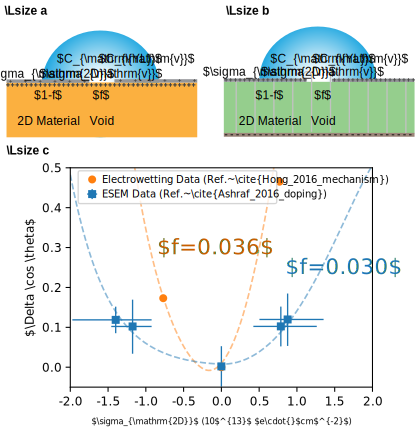
\includegraphics[width=0.95\linewidth]{../img/plot-fitting.pdf}
  \caption{\label{fig:wet-f-nc-exp} Comparison between model and
    experimental data: schemes of the void region in \textbf{a}
    substrated doped 2D material and \textbf{b} electrostatic gated 2D
    material. \textbf{c}. Fitted experimental data of
    \(\Delta\cos\theta\) as a function of
    \(\sigma_{\mathrm{2D}}\). The electrowetting data are extracted
    from Ref. \cite{Hong_2016_mechanism}; the ESEM data are extracted
    from Ref. \cite{Ashraf_2016_doping}.}
\end{figure}

\autoref{fig:wet-f-nc-exp}\lc{a} and \autoref{fig:wet-f-nc-exp}\lc{b} illustrate how
an electric field, either from the dopants on the substrate surface or
from the electrostatic gating, penetrate through a void in a 2D
material sheet and interact with the liquid phase directly. As a
result, the EDL is built up adjacent to the substrate surface, with
the surface excess \(\sigma_{\mathrm{v}}\) and the effective
capacitance \(C_{\mathrm{v}}\).  For molecular doping, the EDL charges
in the void regions are built up by the fixed charges on the substrate
surface, while in the electrostatic doping, the electric field from
the charged 2D material to the gate electrode through the void regions
is responsible for building up the EDL. For both cases, we assume that
\(\sigma_{v}\) is equivalent to \(\sigma_{\mathrm{2D}}\), due to
charge conservation. Together with the EDL and the reorientation
effects discussed earlier, the modified YLE considering a 2D material
with voids follows:
\begin{equation}
\label{eqn:wet-def-Delta-cos-mixture}
\Delta \cos \theta = -f\frac{\sigma_{\mathrm{2D}}^{2}}{\gamma_{\mathrm{L}} C_{\mathrm{v}}} 
                     + (1-f)[(\Delta \cos \theta)^{\mathrm{Orien}} + (\Delta \cos \theta)^{\mathrm{EDL}}]
\end{equation}
where \(f\) is the void (defect) fraction in the 2D material. For the
electrostatic gating experiments (see 
\autoref{fig:wet-f-nc-exp}\lc{a}), the 2D material quantum capacitor
and the dielectric  capacitor are connected in
series, so that the voltage applied between the gate electrode and
2D material, \(V_{\mathrm{G}}\), is given by:
\begin{equation}
\label{eqn:wet-VG-gating}
V_{\mathrm{G}} = \frac{\sigma_{\mathrm{2D}} - \sigma_{\mathrm{0}}}{C_{\mathrm{d}}}
                  + \int_{\sigma_{0}}^{\sigma_{\mathrm{2D}}} \frac{1}{C_{\mathrm{Q}}} \mathrm{d}\sigma'
\end{equation}
where \(C_{\mathrm{d}}\) is the capacitance of the dielectric layer, and
\(\sigma_{0}\) is the initial doping density of the 2D material,
corresponding to \(V_{\mathrm{G}}=0\).


Next, in order to examine the effect of incomplete 2D material
coverage, two independent sets of experimental results, which measure
the water contact angle on (i) substrate-doped graphene
\autocite{Ashraf_2016_doping} and (ii) electrostatically-gated
graphene \autocite{Hong_2016_mechanism} are chosen to compare, with
\(C_{\mathrm{v}} = C_{\mathrm{DH}}\) and \(C_{\mathrm{v}} =
C_{\mathrm{d}}\) in \autoref{eqn:wet-def-Delta-cos-mixture}, respectively. The
parameter \(f\) and \(\sigma_{0}\) are determined by least-square fitting
the experimentally-observed \(\Delta \cos \theta\) with respect to
\(\sigma_{\mathrm{2D}}\) using \autoref{eqn:wet-def-Delta-cos-mixture}. 
\autoref{fig:wet-f-nc-exp}(c) compares the calculated \(\Delta \cos \theta\) as a
function of \(\sigma_{\mathrm{2D}}\), together with the two sets of
experimental data. In both cases considered, we observe a slight
degree of shift in the minima of the fitted curves, corresponding to
the CNP of graphene, or \(\sigma_{\mathrm{2D}} = 0\). In other words, we
observe \(\sigma_{0} = 0\) in both cases, which is typical for
CVD-grown graphene samples
\autocite{Shih_2015_PartiallyScreened,goniszewski_correlation_2016}.  The
fitted values of \(f\) are reasonably small (3.6\% for the
electrostatically-gated graphene and 3.0\% for substrate-doped
graphene), clearly demonstrating that the contact angle change can be
greatly influenced by the defect density. We believe this explains the
discrepancy between the experimental observations and the multiscale
theoretical framework proposed here.

\begin{figure}[!htbp]
  \centering
  \import{\imgdir}{dcos-all-2D.pdf_tex}
% 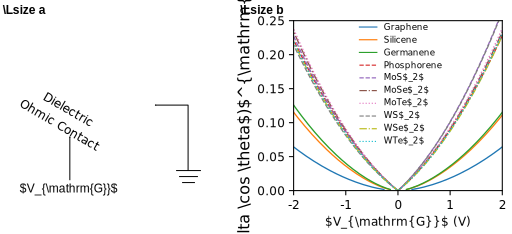
\includegraphics[width=0.65\linewidth]{../img/dcos-all-2D.pdf}
\caption{\label{fig:wet-dcos-all-2D} Electrostatic tunability of 2D
  material wettability: a Schematic illustration of the
  2D-material-based electrowetting device, where the 2D material is
  electostatically doped. b \((\Delta\cos\theta)^{\mathrm{EDL}}\) as
  a function of \(V_{\mathrm{G}}\) for selected 2D materials.}
\end{figure}


Finally, we discuss the influence of 2D material choice under
electrostatic gating condition. The above analysis (eq
\autoref{eqn:wet-Delta-cos-EDL-final}) has clearly suggested that the contact
angle change effect \((\Delta \cos \theta)^{\mathrm{EDL}}\) only depends
on \(\sigma_{\mathrm{2D}}\), which can be controlled by an electric
displacement field, with the experimental setup shown in 
\autoref{fig:wet-dcos-all-2D}\lc{a}. Specifically,  \autoref{eqn:wet-psi-GC} and
\autoref{eqn:wet-VG-gating} suggest:
\begin{equation}
\label{eqn:wet-dVG-choice-2D}
\begin{aligned}
\mathrm{d} V_{\mathrm{G}} &= (\frac{1}{C_{\mathrm{d}}} + \frac{1}{C_{\mathrm{Q}}}) \mathrm{d} \sigma_{\mathrm{2D}} \\
\mathrm{d} \psi_{\mathrm{2D}} &= -(\frac{1}{C_{\mathrm{H}}} + \frac{1}{C_{\mathrm{GC}}}) \mathrm{d} \sigma_{\mathrm{L}}
\end{aligned}
\end{equation}
And since \(\sigma_{\mathrm{2D}} = -\sigma_{\mathrm{L}}\), the first
derivative of \(\psi_{\mathrm{2D}}\) with respect to \(V_{\mathrm{G}}\), namely \(\beta\), is given by:
\begin{equation}
\label{eqn:wet-def-beta}
\beta = \dfrac{\mathrm{d} \psi_{\mathrm{2D}}}{\mathrm{d} V_{\mathrm{G}}} 
= \dfrac{C_{\mathrm{H}}^{-1} + C_{\mathrm{GC}}^{-1}}{C_{\mathrm{d}}^{-1} + C_{\mathrm{Q}}^{-1}}
\end{equation}
The index \(\beta\) here quantifies the tunability of the contact angle change
by \(V_{\mathrm{G}}\). Accordingly, a high degree of \(\beta\) can be attained by increasing both \(C_{\mathrm{d}}\) and
\(C_{\mathrm{Q}}\), thereby introducing the dependence on the choice of 2D material.

Here we demonstrate such phenomenon by considering an electrowetting
setup comprised of a thin, high-\(k\) dielectric layer (2 nm
HfO\(_{\text{2}}\) layer with the relative permittivity
\(\varepsilon_{\mathrm{d}}=24.0\)) underlying a layer of monolayer 2D
material (\autoref{fig:wet-dcos-all-2D}\lc{a}).  As addressed earlier, due
to the fact that \((\Delta \cos \theta)^{\mathrm{Orien}}\) of
graphene-water system may not be readily applied to other 2D
materials, we compare the calculated
\((\Delta \cos \theta)^{\mathrm{EDL}}\) as a function of
\(V_{\mathrm{G}}\), by using the DFT-calculated
\(C_{\mathrm{Q}} - \sigma_{\mathrm{2D}}\) relations for a variety of
2D materials, as shown in \autoref{fig:wet-dcos-all-2D}\lc{b}. Clearly, as a
consequence of the high quantum capacitance, the wettability of the 2D
semiconductors considered is more tunable compared to that for the 2D
semimetals under same the applied gate voltage. In other words, in a 2D
semiconductor, the value required to reach a certain is lowered. We
predict that the contact angle change \(\Delta \cos \theta\) for the
2D semiconductors (e.g. TMDCs) can reach up to
0.22\textasciitilde{}0.25 within the range of \(V_{\mathrm{G}}\)
considered, corresponding to an interfacial tension change of
15\textasciitilde{}18 \(\mathrm{mJ} \cdot \mathrm{m}^{-2}\). The
analysis presented here suggests that the manipulation of a liquid
droplet on a layer of 2D material doped by an electric displacement
field may be feasible \autocite{Mugele_2005_EW_rev,Hayes_2003_nature_EWOD}.

An interesting implication is that, together with the recent
development in engineering 2D materials’ wetting translucency
\autocite{Raj_2013_wetting_rev,rafiee_2012_transparency,Shih_2012_prl,shih_2013_wetting_natmat},
in principle, upon doping, a 2D material becomes less “transparent” (or more screening)
to both van der Waals and Coulombic interactions exerted from the underlying
substrate, due to enhanced liquid-2D material interactions. That is to say, the doping level can be
another control variable to modulate the molecular packing and
epitaxial behavior on a 2D material-coated surface, which may bring
new technological opportunity for a variety of applications.


\section{Conclusions}
\label{sec:wet-conclusions}

In this chapter, we present a multiscale theoretical framework
concerning the wettability of doped 2D materials, by considering: (i)
the change of 2D materials surface energy, (ii) the molecular
reorientation of liquid molecules adjacent to the interface, and (iii)
the electrical double layer formed in the liquid phase. Taking
graphene as an example, we show that the Coulombic interaction
dominates the change of liquid-2D material interfacial tension, at
both molecular and mesoscopic length scales. The latter two effects were
found to be the major mechanisms responsible for the water contact angle
change at the 2D material interfaces upon doping.

The doping-induced reorientation of liquid molecules at the
graphene-liquid interface is revealed by MD simulations. It is
found that the interfacial energy change is dominated by the Coulombic
interactions. Our results also reveal an asymmetric change of
graphene-water interfacial energy upon doping, such that slightly
n-doped graphene can reorient interfacial water molecules to minimize
electrostatic attractions, and therefore, slightly increase the
interfacial energy. 
%
On the other hand, the EDL effect is calculated by a continuum model. Our
analysis suggests that the reorientation effect is more predominant
than the EDL effect. On the graphene-water interface, we predict that
the combined reorientation and EDL effects can induce a significant
change of the interfacial tension \(\Delta
\gamma_{\mathrm{2D-L}}\), up to -15 \(\mathrm{mJ}\cdot
\mathrm{m}^{-2}\), at the doping level of \(\pm 4 \times 10^{13}\ e\cdot
\mathrm{cm}^{-2}\). By adding the fitting parameter concerning the
defect density, our theoretical framework can nicely describe the
experimentally observed doping-induced contact angle change. Finally,
based on the DFT-calculated quantum capacitances (QCs) for a variety
of 2D materials, we predict that the wettability of 2D semiconductors
(e.g., TMDCs) is more tunable under an electric displacement field,
compared with 2D semimetals (e.g. graphene) due to their high quantum
capacitances. Our findings reveal a complete picture for the
modulation of the molecular interactions between liquid and a 2D monolayer upon
doping. The multiscale theoretical
framework proposed here is expected to shed
light on the surface science of 2D materials, 
as well as to provide a quantitative estimation for the wettability
of the doped 2D materials. 

\section{Methods}
\label{sec:wet-methods}

\subsection*{MD Simulations}
\label{sec:wet-md-simulations}


All MD simulations were carried out
using the \texttt{GROMACS} 4.5 software package
\autocite{Hess_2008_gromacs}. Monolayer graphene was modeled as an
infinite rigid sheet in the \textit{xy}-plane.
%
The carbon atoms of graphene were treated as Lennard-Jones (LJ)
spheres with \(\sigma\) = 0.34 nm and \(\epsilon\) = 0.223 kJ/mol
\autocite{Cheng_1990}, such that the pair-wise LJ potential
$w_{\mathrm{LJ}}$ is calculated by
\(w_{\mathrm{LJ}} = 4
\epsilon\left[\left(\dfrac{\delta}{r}\right)^{12} -
  \left(\dfrac{\delta}{r}\right)^{6}\right]\), where $r$ is the
distance.  The force-field parameters are adapted from reports by
Tummala and Striolo \autocite{Tummala_2008_counterion_SDS}.
%
The doping effect is included by assigning an equal amount of charge
\(\sigma_{\mathrm{2D}} / \rho_{\mathrm{G}}\), where
\(\rho_{\mathrm{G}}\) is the surface density of carbon in graphene, to
each atom.
%
The range of \(\sigma_{\mathrm{2D}}\) considered here
approximately corresponds to the partial atomic charge from −0.012 to
0.012 \(e/\mathrm{atom}\).
%
Water molecules were modeled using the SPC/E model
\autocite{Berendsen_1987_pair} with bond lengths and angles constrained
using the \texttt{SETTLE} algorithm
\autocite{Miyamoto_1992_SHAKE_RATTLE}. Lennard-Jones interactions were
treated with a cutoff distance of 1 nm, with those between different
atoms calculated using the standard geometric averaging
rule. Long-range electrostatic interactions were treated using the
particle mesh Ewald (PME) summation method
\autocite{Darden_1993_ewald,Essmann_1995_ewald} with a short-range cutoff
distance of 1 nm. The velocity-rescaled Berendsen thermostat was
implemented to maintain a constant system temperature of 298.15 K
\autocite{Bussi_2007}. All simulations were carried out under the NVT
ensemble, and the equations of motion of water molecules were
integrated over a range of 20 ns with 10\(^{\text{7}}\) steps.

Periodic boundary conditions are used in all three directions of the
simulation boxes in both systems. Additionally, a vacuum layer of 3 nm
thick along the \emph{z}-axis is placed to separate the periodic
images of the graphene-water system. A simulation box with a
sufficiently large length of 21 nm in the \emph{z}-direction is used,
with a 18-nm thick block of water molecules, to minimize the effect of
the long-range electrostatic interaction between the charged graphene
and the water molecules at the water-vacuum interface, by ensuring
that the time-averaged dipole moment for the water molecules at the
water-vacuum interface approaches zero.




\section{Author Contributions}
\label{sec:wet-author-contributions}

T.T. and C.J.S. designed the theoretical study and
simulations. T.T. and C.J.S. derived the analytical solutions for the
surface energy change of isolated 2D material and pure EDL effect. MD
simulations were performed by L.Z. and S.L. and data analysis done
jointly by T.T. and S.L. All authors contribute to the discussions.






% \bibliography{ref}




%%% Local Variables:
%%% mode: latex
%%% TeX-master: "../thesis"
%%% End:
